\subsection{All four cuts, against the curvature mismatch}
\label{sec:dkappa}

% Four-cut summary, drawn from the logged numbers.
% The script's own summary PNG covers only the three cuts of one process,
% because cut 1 was run separately; this figure carries all four.
\begin{figure}[htbp]
\centering
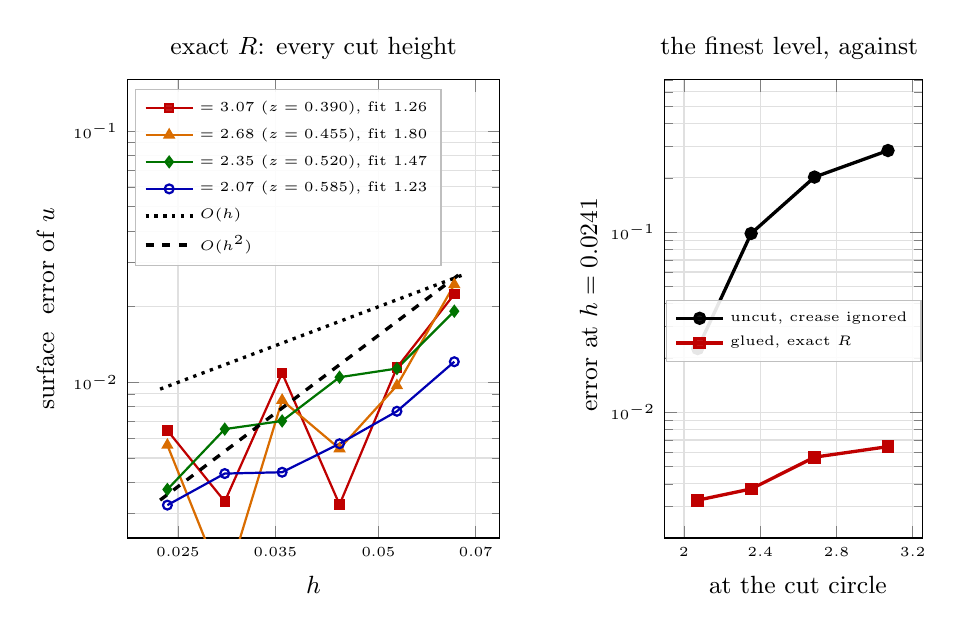
\begin{tikzpicture}

\begin{loglogaxis}[
  name=left,
  width=0.52\textwidth, height=7.4cm,
  xlabel={$h$}, ylabel={surface $\Linf$ error of $u$},
  title={\small exact $R$: every cut height},
  title style={yshift=-2pt},
  legend style={font=\tiny, at={(0.02,0.98)}, anchor=north west,
                draw=black!25, fill=white, fill opacity=0.9,
                text opacity=1, legend columns=1, row sep=0.5pt},
  legend cell align=left,
  xmin=0.021, xmax=0.076, ymin=2.4e-3, ymax=0.16,
  grid=both, grid style={black!12},
  tick label style={font=\tiny}, label style={font=\small},
  xtick={0.025,0.035,0.05,0.07},
  xticklabels={0.025,0.035,0.05,0.07},
]

\addplot[red!75!black, thick, mark=square*, mark size=1.5]
  coordinates {
    (0.065,2.244e-2) (0.053300,1.145e-2) (0.043706,3.261e-3)
    (0.035839,1.089e-2) (0.029388,3.356e-3) (0.024098,6.436e-3)};
\addlegendentry{$\dk=3.07$ ($z=0.390$), fit 1.26}

\addplot[orange!85!black, thick, mark=triangle*, mark size=1.8]
  coordinates {
    (0.065,2.451e-2) (0.053300,9.706e-3) (0.043706,5.444e-3)
    (0.035839,8.485e-3) (0.029388,1.516e-3) (0.024098,5.624e-3)};
\addlegendentry{$\dk=2.68$ ($z=0.455$), fit 1.80}

\addplot[green!45!black, thick, mark=diamond*, mark size=1.8]
  coordinates {
    (0.065,1.920e-2) (0.053300,1.135e-2) (0.043706,1.048e-2)
    (0.035839,7.020e-3) (0.029388,6.515e-3) (0.024098,3.747e-3)};
\addlegendentry{$\dk=2.35$ ($z=0.520$), fit 1.47}

\addplot[blue!70!black, thick, mark=o, mark size=1.6]
  coordinates {
    (0.065,1.208e-2) (0.053300,7.672e-3) (0.043706,5.697e-3)
    (0.035839,4.387e-3) (0.029388,4.334e-3) (0.024098,3.245e-3)};
\addlegendentry{$\dk=2.07$ ($z=0.585$), fit 1.23}

\addplot[black, dotted, very thick, domain=0.0235:0.067, samples=2]
  {2.6e-2*x/0.065};
\addlegendentry{$O(h)$}

\addplot[black, dashed, very thick, domain=0.0235:0.067, samples=2]
  {2.6e-2*(x/0.065)^2};
\addlegendentry{$O(h^2)$}

\end{loglogaxis}

\begin{semilogyaxis}[
  name=right, at={(left.east)}, anchor=west, xshift=2.1cm,
  width=0.40\textwidth, height=7.4cm,
  xlabel={$\dk$ at the cut circle},
  ylabel={$\Linf$ error at $h=0.0241$},
  ylabel style={yshift=-2pt},
  title={\small the finest level, against $\dk$},
  title style={yshift=-2pt},
  legend style={font=\tiny, at={(0.5,0.52)}, anchor=north,
                draw=black!25, fill=white, fill opacity=0.9,
                text opacity=1},
  legend cell align=left,
  xmin=1.9, xmax=3.25, ymin=2e-3, ymax=0.7,
  grid=both, grid style={black!12},
  tick label style={font=\tiny}, label style={font=\small},
  xtick={2.0,2.4,2.8,3.2},
]

\addplot[black, very thick, mark=*, mark size=1.8]
  coordinates {(2.0720,2.255e-2) (2.3525,9.824e-2)
               (2.6849,2.020e-1) (3.0703,2.836e-1)};
\addlegendentry{uncut, crease ignored}

\addplot[red!75!black, very thick, mark=square*, mark size=1.7]
  coordinates {(2.0720,3.245e-3) (2.3525,3.747e-3)
               (2.6849,5.624e-3) (3.0703,6.436e-3)};
\addlegendentry{glued, exact $R$}

\end{semilogyaxis}

\end{tikzpicture}
\caption{All four cut heights. Left: the surface $\Linf$ error of the
  glued solve with the exact rotation, against $h$. The uncut baseline is
  left out of this panel, because it is two orders of magnitude higher;
  it appears in Figure~\ref{fig:cut039} and in the right panel here. All
  four glued curves sit between the $O(h)$ and $O(h^2)$ guides, and all
  four zigzag. Right: the error at the finest level, against the
  curvature mismatch $\dk$. Both the baseline and the glued solve order
  monotonically by $\dk$, although the \emph{fitted slopes} do not ---
  see the text below.}
\label{fig:cutsummary}
\end{figure}


The four cut heights span crease angles from $34.9^\circ$ to
$81.8^\circ$, and with them a range of curvature mismatch.
Table~\ref{tab:fourcuts} collects them.

\begin{table}[htbp]
\centering
\caption{All four cuts of the flipped ellipsoid. $\dk$ falls as the cut
  moves from the equator towards the pole. Each entry is the fitted
  slope over six levels, with the error at the finest level
  ($h=0.0241$) beside it.}
\label{tab:fourcuts}
\footnotesize
\setlength{\tabcolsep}{4pt}
\begin{tabular}{@{}rrcrr rr rr rr rr@{}}
\toprule
 & & & &
 & \multicolumn{2}{c}{uncut, crease ignored}
 & \multicolumn{2}{c}{$d_k$}
 & \multicolumn{2}{c}{$d_{k2}$}
 & \multicolumn{2}{c}{exact $R$} \\
\cmidrule(lr){6-7}\cmidrule(lr){8-9}\cmidrule(lr){10-11}\cmidrule(lr){12-13}
$z$ & $\varphi_c$ & crease & $\kappa_m$ & $\dk$
 & rate & error & rate & error & rate & error & rate & error \\
\midrule
0.390 & 0.9273 & $81.8^\circ$ & 1.2986 & 3.0703
 & 0.10 & 2.84e-01 & 1.20 & 6.45e-03 & 2.31 & 6.41e-03 & 1.26 & 6.44e-03 \\
0.455 & 0.7954 & $67.1^\circ$ & 1.0970 & 2.6849
 & 0.59 & 2.02e-01 & 1.78 & 5.60e-03 & 2.20 & 5.80e-03 & 1.80 & 5.62e-03 \\
0.520 & 0.6435 & $52.0^\circ$ & 0.9220 & 2.3525
 & 0.33 & 9.82e-02 & 1.47 & 3.74e-03 & 1.89 & 3.70e-03 & 1.47 & 3.75e-03 \\
0.585 & 0.4510 & $34.9^\circ$ & 0.7738 & 2.0720
 & 1.00 & 2.25e-02 & 1.22 & 3.26e-03 & 1.22 & 3.28e-03 & 1.23 & 3.24e-03 \\
\bottomrule
\end{tabular}
\end{table}

\paragraph{The error level orders by $\dk$. The fitted rate does not.}
This is the main qualification on this test. At the finest level the
error of the glued solve falls monotonically as $\dk$ falls:
\begin{equation*}
  6.44,\quad 5.62,\quad 3.75,\quad 3.25 \;\;(\times 10^{-3})
  \qquad\text{for}\qquad
  \dk = 3.07,\; 2.68,\; 2.35,\; 2.07 .
\end{equation*}
The uncut baseline does the same, and far more strongly: from
$2.84\times10^{-1}$ down to $2.25\times10^{-2}$, a factor of 12.

The fitted slopes, by contrast, are $1.26$, $1.80$, $1.47$ and $1.23$.
They do not order by $\dk$, and they do not order by anything else
either. Six levels are not enough to separate a trend in the rate from
the grid-alignment scatter of Section~\ref{sec:scatter}. The defensible
statement from this study is therefore:

\begin{quote}
  Every cut converges at a fitted rate between $1.2$ and $1.8$. None
  reaches second order. The size of the error at a fixed grid spacing
  grows with $\dk$, as Equation~\eqref{eq:bound3} says it should ---
  through the constant in $C\,h\,D$, not through the exponent.
\end{quote}

That is how a bound behaves when its junction term is first order with a
$\dk$-dependent constant. Changing $\dk$ moves the curve up and down. It
would change the \emph{rate} only if $\dk$ reached zero. The unflipped
cut, where $\dk$ vanishes identically, is the test of that. It is the
\texttt{flipped = false} branch of the script, and it is not run here.

\paragraph{Where the error sits.} The script reports the distance of the
worst point from the cut circle, in units of $h$. At the two sharpest
cuts that distance is within one cell at nearly every level. At the
mildest cut, $z=0.585$, it is $11.5$, $14.1$ and $16.6$ cells at the
three coarsest levels, and it moves to the crease only at the three
finest. At a mild crease the junction is not the worst thing in the
solve until the grid is fine enough for the interior error to fall below
it.

\paragraph{The estimated rotations, across all cuts.} At every cut the
three variants agree at the finest level to within 1 per cent. The
fitted rates of the angle error are $2.13$, $2.30$, $2.36$ and $1.98$
for $d_k$, and $3.60$, $3.25$, $3.76$ and $2.93$ for $d_{k2}$. Both
estimators beat the nominal order of their underlying difference at
every cut, and neither difference reaches the solution.
